\documentclass[14pt]{extbook}
\usepackage{multicol, enumerate, enumitem, hyperref, color, soul, setspace, parskip, fancyhdr} %General Packages
\usepackage{amssymb, amsthm, amsmath, latexsym, units, mathtools} %Math Packages
\everymath{\displaystyle} %All math in Display Style
% Packages with additional options
\usepackage[headsep=0.5cm,headheight=12pt, left=1 in,right= 1 in,top= 1 in,bottom= 1 in]{geometry}
\usepackage[usenames,dvipsnames]{xcolor}
\usepackage{dashrule}  % Package to use the command below to create lines between items
\newcommand{\litem}[1]{\item#1\hspace*{-1cm}\rule{\textwidth}{0.4pt}}
\pagestyle{fancy}
\lhead{Progress Quiz 9}
\chead{}
\rhead{Version C}
\lfoot{9541-5764}
\cfoot{}
\rfoot{Summer C 2021}
\begin{document}

\begin{enumerate}
\litem{
First, find the equation of the line containing the two points below. Then, write the equation in the form $ y=mx+b $ and choose the intervals that contain $m$ and $b$.\[ (-7, -2) \text{ and } (-10, 8) \]\begin{enumerate}[label=\Alph*.]
\item \( m \in [3.33, 4.33] \hspace*{3mm} b \in [36.33, 45.33] \)
\item \( m \in [-7.33, 2.67] \hspace*{3mm} b \in [18, 20] \)
\item \( m \in [-7.33, 2.67] \hspace*{3mm} b \in [18.33, 31.33] \)
\item \( m \in [-7.33, 2.67] \hspace*{3mm} b \in [-28.33, -23.33] \)
\item \( m \in [-7.33, 2.67] \hspace*{3mm} b \in [1, 7] \)

\end{enumerate} }
\litem{
Solve the equation below. Then, choose the interval that contains the solution.\[ -8(-18x + 9) = -3(10x -16) \]\begin{enumerate}[label=\Alph*.]
\item \( x \in [0.66, 0.74] \)
\item \( x \in [0.08, 0.16] \)
\item \( x \in [0.18, 0.26] \)
\item \( x \in [-0.16, -0.11] \)
\item \( \text{There are no real solutions.} \)

\end{enumerate} }
\litem{
Solve the equation below. Then, choose the interval that contains the solution.\[ -6(18x + 2) = -10(5x + 17) \]\begin{enumerate}[label=\Alph*.]
\item \( x \in [-1.74, -0.02] \)
\item \( x \in [2.73, 3.93] \)
\item \( x \in [-3.5, -2.9] \)
\item \( x \in [1.45, 3.12] \)
\item \( \text{There are no real solutions.} \)

\end{enumerate} }
\litem{
First, find the equation of the line containing the two points below. Then, write the equation in the form $ y=mx+b $ and choose the intervals that contain $m$ and $b$.\[ (-8, -4) \text{ and } (4, 4) \]\begin{enumerate}[label=\Alph*.]
\item \( m \in [0.3, 3.3] \hspace*{3mm} b \in [-0.77, 1.26] \)
\item \( m \in [0.3, 3.3] \hspace*{3mm} b \in [3.59, 4.14] \)
\item \( m \in [0.3, 3.3] \hspace*{3mm} b \in [0.04, 1.6] \)
\item \( m \in [-2.1, -0.3] \hspace*{3mm} b \in [6.35, 6.99] \)
\item \( m \in [0.3, 3.3] \hspace*{3mm} b \in [-1.61, -0.27] \)

\end{enumerate} }
\litem{
Find the equation of the line described below. Write the linear equation in the form $ y=mx+b $ and choose the intervals that contain $m$ and $b$.\[ \text{Perpendicular to } 4 x - 5 y = 7 \text{ and passing through the point } (-8, 4). \]\begin{enumerate}[label=\Alph*.]
\item \( m \in [-2.28, -1.2] \hspace*{3mm} b \in [12, 13] \)
\item \( m \in [-0.19, 1.43] \hspace*{3mm} b \in [14, 16] \)
\item \( m \in [-2.28, -1.2] \hspace*{3mm} b \in [-13, -5] \)
\item \( m \in [-2.28, -1.2] \hspace*{3mm} b \in [3, 8] \)
\item \( m \in [-1.11, 0.29] \hspace*{3mm} b \in [-13, -5] \)

\end{enumerate} }
\litem{
Write the equation of the line in the graph below in Standard Form $Ax+By=C$. Then, choose the intervals that contain $A, B, \text{ and } C$.
\begin{center}
    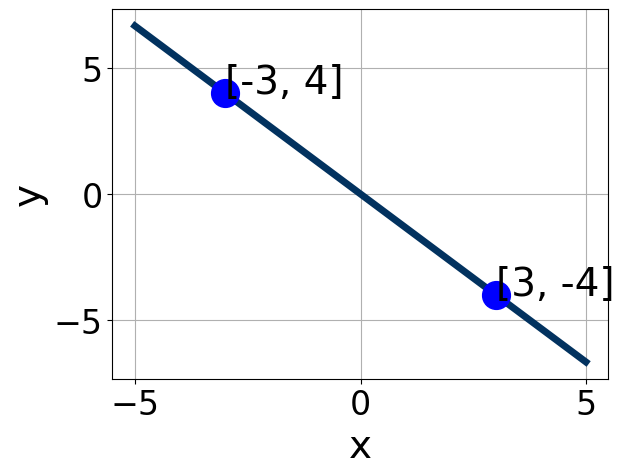
\includegraphics[width=0.5\textwidth]{../Figures/linearGraphToStandardC.png}
\end{center}
\begin{enumerate}[label=\Alph*.]
\item \( A \in [-5.1, -1.8], \hspace{3mm} B \in [-4.02, -2.14], \text{ and } \hspace{3mm} C \in [-6, 2] \)
\item \( A \in [-0.5, 2.4], \hspace{3mm} B \in [0.14, 2.7], \text{ and } \hspace{3mm} C \in [-6, 2] \)
\item \( A \in [2.8, 6.2], \hspace{3mm} B \in [-4.02, -2.14], \text{ and } \hspace{3mm} C \in [-6, 2] \)
\item \( A \in [-0.5, 2.4], \hspace{3mm} B \in [-1.95, 0.43], \text{ and } \hspace{3mm} C \in [-6, 2] \)
\item \( A \in [2.8, 6.2], \hspace{3mm} B \in [2.21, 3.98], \text{ and } \hspace{3mm} C \in [-6, 2] \)

\end{enumerate} }
\litem{
Solve the linear equation below. Then, choose the interval that contains the solution.\[ \frac{-5x -4}{7} - \frac{-3x + 8}{3} = \frac{6x -9}{8} \]\begin{enumerate}[label=\Alph*.]
\item \( x \in [-5.2, -3.2] \)
\item \( x \in [-1.7, 0.7] \)
\item \( x \in [-7.3, -5.8] \)
\item \( x \in [5.9, 7.5] \)
\item \( \text{There are no real solutions.} \)

\end{enumerate} }
\litem{
Solve the linear equation below. Then, choose the interval that contains the solution.\[ \frac{-5x + 3}{5} - \frac{-9x + 9}{7} = \frac{9x + 9}{8} \]\begin{enumerate}[label=\Alph*.]
\item \( x \in [-2.3, -0.9] \)
\item \( x \in [-18.2, -17.2] \)
\item \( x \in [0.4, 1.8] \)
\item \( x \in [-2, 0.1] \)
\item \( \text{There are no real solutions.} \)

\end{enumerate} }
\litem{
Write the equation of the line in the graph below in Standard Form $Ax+By=C$. Then, choose the intervals that contain $A, B, \text{ and } C$.
\begin{center}
    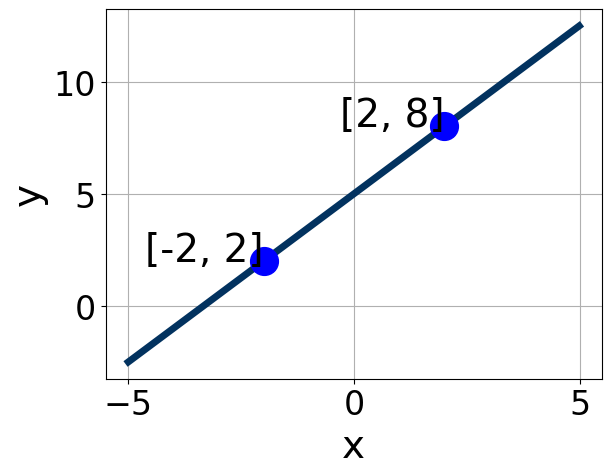
\includegraphics[width=0.5\textwidth]{../Figures/linearGraphToStandardCopyC.png}
\end{center}
\begin{enumerate}[label=\Alph*.]
\item \( A \in [-5.4, -2.4], \hspace{3mm} B \in [1.11, 3.02], \text{ and } \hspace{3mm} C \in [6, 11] \)
\item \( A \in [-2, -1.4], \hspace{3mm} B \in [-1.36, -0.52], \text{ and } \hspace{3mm} C \in [-6, -3] \)
\item \( A \in [-2, -1.4], \hspace{3mm} B \in [0.67, 1.45], \text{ and } \hspace{3mm} C \in [4, 7] \)
\item \( A \in [1.6, 5.1], \hspace{3mm} B \in [1.11, 3.02], \text{ and } \hspace{3mm} C \in [6, 11] \)
\item \( A \in [1.6, 5.1], \hspace{3mm} B \in [-2.35, -1.69], \text{ and } \hspace{3mm} C \in [-14, -7] \)

\end{enumerate} }
\litem{
Find the equation of the line described below. Write the linear equation in the form $ y=mx+b $ and choose the intervals that contain $m$ and $b$.\[ \text{Perpendicular to } 6 x - 5 y = 12 \text{ and passing through the point } (9, 5). \]\begin{enumerate}[label=\Alph*.]
\item \( m \in [-1.37, -1.11] \hspace*{3mm} b \in [11.5, 14.5] \)
\item \( m \in [0.34, 1.39] \hspace*{3mm} b \in [-3.5, -1.5] \)
\item \( m \in [-0.93, -0.78] \hspace*{3mm} b \in [-12.5, -11.5] \)
\item \( m \in [-0.93, -0.78] \hspace*{3mm} b \in [-5, -3] \)
\item \( m \in [-0.93, -0.78] \hspace*{3mm} b \in [11.5, 14.5] \)

\end{enumerate} }
\end{enumerate}

\end{document}